\documentclass[tikz,border=0.5cm,12pt]{standalone}
\usepackage[fontsize=16pt]{fontsize}
\usepackage{util}
\usetikzlibrary{shapes.multipart}

\begin{document}
  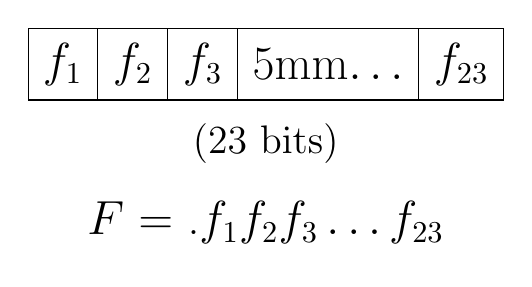
\begin{tikzpicture}[boxes/.style={draw,rectangle split,rectangle split parts=#1,anchor=center}]
    \node [name=diagram, boxes=5, rectangle split horizontal] at (0, 0) {
      \nodepart{one} $f_1$
      \nodepart{two} $f_2$
      \nodepart{three} $f_3$
      \nodepart{four} \pad{5mm}{$\dots$}
      \nodepart{five} $f_{23}$
    };

    \draw[shift=(diagram.south)]
      node[below=1mm] {\small (23 bits)};
    \draw[shift=(diagram.south)]
      node[below=(14pt + 6mm)] {$F$ = .$f_1 f_2 f_3 \dots f_{23}$};
  \end{tikzpicture}
\end{document}
